\documentclass{standalone}

\usepackage{tikz}
\usepackage{circuitikz}

\tikzset{block/.style = {draw, fill=white, very thick, rectangle, minimum height=1cm, minimum width=2cm},
         lblock/.style={draw,fill=white,very thick, rectangle, minimum height=3cm, minimum width=1cm},
         sum/.style= {draw, fill=white, very thick, circle, node distance=0.5cm}}

         
\begin{document}
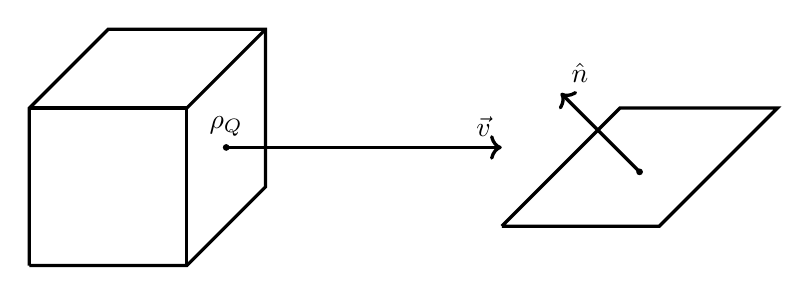
\begin{tikzpicture}[scale=2]
    \draw[-,very thick](0,0)--(1,0)--(1.5,0.5)--(1.5,1.5)--(0.5,1.5)--(0,1)--(0,0);
    \draw[-,very thick](1,0)--(1,1)--(0,1);
    \draw[-,very thick](1,1)--(1.5,1.5);

    \draw[->,very thick](1.25,0.75)node[above]{$\rho_Q$}--(3,0.75)node[above left]{$\vec{v}$};

    \draw[-,very thick](3,0.25)--(3.75,1)--(4.75,1)--(4,0.25)--(3,0.25);
    \draw[->,very thick](3.875,0.595)--(3.375,1.095)node[above right]{$\hat{n}$};
    \filldraw[black](3.875,0.595)circle(0.5pt);
    \filldraw[black](1.25,0.75)circle(0.5pt);
\end{tikzpicture}
\end{document}